In this chapter we present some background related to analytic in the domain of soccer. We look at different types of analysis out there. This spans from pre-match to post-match. Then we go into how data is gathered and presented. For gathering of data there are two main approaches: manually often by human annotating it, and automatic capturing often by using sensors.

\section{Types of analysis}

In soccer there are several phases where you use analytic to help you gain insight.  In this section we will look at the typical use cases of analytic. Not only soccer teams uses analytics, but also TV and fans widely uses statistics to build up under their arguments.

\subsection{Pre-match}

Pre-match you use analytic to find weaknesses and strengths in the opponent team, on an individually level or as a team. You look at your team matched up against your opponent. A typical situation is that the manager gets a video summary of the opponent highlighting the opponent’s strengths and weaknesses. The coaching staff may use tools like Interplay to gather information and create the video summary. Other software like Prozone\ref{http://www.prozonesports.com/index.html} will also likely be used to break down the opponents offensive and defensive play. 

Typically in TV you have pundits bringing you analytic of key battles during the build up to the game. A typical thing is to look at battles like wingers versus backs, midfield clashes or striker versus central defenders. The battles are often illustrated with statistics or with video clips highlighting aspects of the both players game that will be decisive. 

Fans are analyzing the game all the time. Except from TV they get exposed to analytic via social media. Opta is company that has taken full advantage of social medias. Figure \ref{fig:optastats.png} is a screenshot of a tweet from one of the many accounts Opta control. 

\begin{figure}[ht!]
\centering
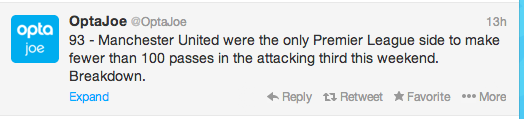
\includegraphics[width=1\textwidth]{images/general/optastats.png}
\caption{A typical tweet from one of Opta's Twitter account}
\label{fig:optastats}
\end{figure}

\subsubsection{In match}

During match the coaching staff continuously analysis the match and makes adjustment. The players make all the decisions in the end, but the coach is the boss and sets the style of play. An adjustment to the formation can potentially be the tipping point that wins you the game.

Tromsø IL uses a system Muithu that lets you annotate sequences of a game with entity's like player, comment. This information will then be time synchronized with the video feed. Later, like in at half time or even in the game, you can search on entity's to get the corresponding video feed. As the system is available on tablets players can in the middle of the match come to sideline to see a involvement that the coaching staff would like to show. It can be anything that is tagged like a player involvement to a team move that was executed perfectly. 

Using systems like ZXY or MiCoach you can get real time information about a players performance during the match. Rather than assuming that a player is tiring you can get information metrics that tells you this. You get evidence that the player in fact is fatigued. In soccer you only have 3 substitutions. Making the right ones is crucial in an even match.

Using data gathered from sports data company's like Opta you can get statistics live during the game. Its popular in TV to show statistics like ball possession percent, how far players have run or the number of passes played and so on. As mentioned earlier Opta posts many of their statistics to their social media accounts for fans and media.

\subsection{Post match}

During the post match the coach team goes through the game to evaluate the team performance. This is valuable as you get concrete clips about good and bad involvements on team or player level. You can highlight situations in the match to help players better understand tactical aspects. Interplay Sports is a system used today at Alfheim for this purpose. It is used for analysis of matches in a post-match scenario where you can tag situations in the video. 

\section{Capturing of data}
\subsection{Opta}

One of the big players in the field of sport analytic Opta uses manual input to create their data repository. They have editorial teams across the world that captures data manually for the most popular soccer leagues and other sports. For example to capture statistics for a single match they have 3 humans annotating. The data is captured via an application specifically created for the purpose of capturing data as quick and easily as possible. The editorial teams of Opta need to be able to identify a player in a very short time to be able to keep up with the pace of the game. They even study things like which shoe color a player.

Opta capture all types of actions like passes, type of pass, attacks, and interceptions to mention a few. For each action they log, they add a series of description tags like pitch coordinate, timestamp, which player and team. For every single pass they add descriptors if it was a through ball, normal ball or a headed flick on from a long ball. For shots they register the foot it was kicked with, if it was a volley and so on. All this is done while the match is playing. About 1600 individual events are recorded in a standard match.  This gives them a very rich database of events and a range of possible queries to run. 

\begin{lstlisting}
<Event id="290575408" event_id="5" type_id="1" period_id="1" 
min="0" sec="5" player_id="20856" team_id="810" outcome="1" 
x="44.6"y="61.1" timestamp="2007-08-12T13:00:24.827" 
last_modified="2007-08-12T13:00:25">
<Q id="1774596260" qualifier_id="141" value="91.6"/>
<Q id="1429253465" qualifier_id="140" value="49.9"/>
<Q id="1084400575" qualifier_id="56" value="Back"/>
</Event>
\end{lstlisting}

Above is an example of an event registrated in the Opta database. The event has a series of qualifiers describing it. Except from the obvious as timestamp and last modified dates we see that the player id, team id, time of event, x and y coordinates and the outcome of the event are registrated. Also we see that some extra details are included. In this example it maps to a pass from [44.6, 61.1] to [91.6, 49.9]. 

\subsection{Prozone}

Prozone is a video-based system that tries to track players in team sports \cite{Prozone:indepth}. Their data capture system incorporates 8-12 cameras, which is strategically positioned throughout the stadium to cover 100 percent of the ground, but with some redundancy in case of a faulty component. They also incorporate the TV-camera feed, which always follows the ball. All cameras are hooked into one server and uploaded at the end of the game before sent to undertake the tracking process. When they system is installed it required some setup before it is operational; cameras need to be calibrated out from the pitch size. Figure \ref{fig:prozonecam} shows the camera location on a soccer stadium.

\begin{figure}[ht!]
\centering
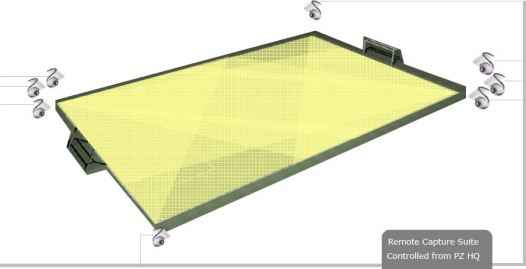
\includegraphics[width=1\textwidth]{images/general/prozonecam.png}
\caption{The Prozone camera system illustrated. Taken from Prozonesports.com}
\label{fig:prozonecam}
\end{figure}

The coding and tracking process of the player's movement and actions is a sort of manual process at present time. First each camera feed goes through each own tracking process determining image co-ordinates and continuous trajectories for each player. The output from all the cameras is then combined into one dataset. Going into the algorithm for this is out of the scope of this project. In the final stage the manual work comes into the loop. There has to be a quality control group of operators dedicated for post processing the game. First the operators has to map the players identity and with the their corresponding start location. The operators will then follow the video feed checking that the identification of all players remains constant during the match. The tracking process may run into problems when two players collide or have any other physical contact as it becomes unclear who is who. To map video image co-ordinates to pitch co-ordinates Prozone uses computer vision homography calibration process.

The whole input process is done in a own software which helps you minimize the amount of manual work for the operators. The software follows rules created by basic machine learning algorithms to validate and verify the input. A simple example would be if the ball goes out of play the system will now that the next event will be a throw in, corner kick or goal kick.

Prozone claims to be able to track every movement of every player on the pitch with a resolution of 10th of a second. This without using any physical equipment on the players. Di Salvo et al. \cite{Prozone:validation} conducted an empirical evaluation of deployed Prozone systems at Old Trafford in Manchester and Reebook Stadium in Bolton, and concluded that the video camera deployment gives an accurate and valid motion analysis. The data is after a match available through Prozone interface for analysis. 

\subsection{Automatic capturing}

A system that uses sensors is the ZXY sport tracking system \footnote{http://www.zxy.no}. The system is in used by premier league soccer teams in Norway, including Tromsø IL and Rosenborg BK. Data captured is stored in Sybase databases with each match requiring about 500-700MB storage The players have to wear a belt around their waist for the system to be able to track their movements. The ZXY system is able to track the player’s movement very detailed with an accuracy of 0.5m. It has a resolution of 20 samples per second. The technology behind it relies on a radio-based signaling substrate to provide real-time high-precision positional tracking, also including acceleration and heart rate. An installation of receivers is required for the system to work. The home arena for Tromsø IL, Alfheim, is currently equipped with 10 receivers. A receiver tracks a specific area of the soccer field and combined they cover the whole pitch with some redundancy areas. The communication from the belt to the receivers goes on a 2.45-5.2 G Hz frequency radio signal. To compute the positional data the stationary radio receiver uses an advance vector based processing of the received radio signal. The data is aggregated and stored into a relational database. Including the positions of the players the ZXY also gives you the step frequency and speed. 

\begin{figure}[ht!]
\centering
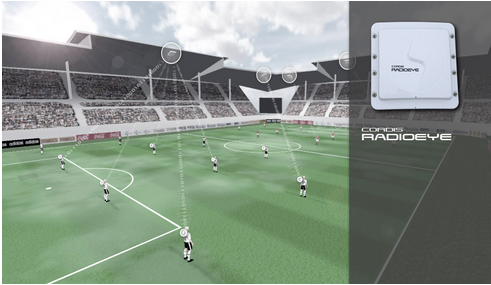
\includegraphics[width=1\textwidth]{images/general/zxyoverview.png}
\caption{Overview of the ZXY system with receivers placed at the stadium and players wearing sensors. Image from zxy.no}
\label{fig:zxycam}
\end{figure}

\subsection{Wrap up}
The main problem with tracking systems that uses physical sensors is that usually only one of the teams wears the sensors. This limits the functionality of the system as an opponent analysis system. You only get data for one team and if you have installed it at your stadium it captures only half of the matches. 

On the other hand you have the manually systems that requires human annotation of matches. These systems have the advantage of being able to track both teams. As they rely on human annotation of some degree they get more rich data as well, but requires strict rules of the semantics of the metadata. 

\section{Presenting data}

This sections gives an short overview of how some systems presents opponent analysis.

\subsection{Prozone}

Prozone comes with several softwares to illustrate the data. The most relevant for this project is the opposition analysis system. It includes features like 2D animation, single player analysis, team analysis, pressing analysis, success/direction, player tempo, passing movements, receving the ball, player events.

\begin{figure}[ht!]
\centering
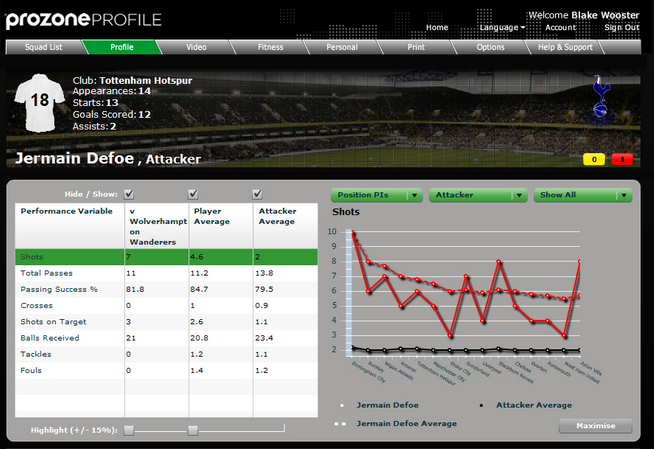
\includegraphics[width=1\textwidth]{images/general/prozonestats.png}
\caption{The Prozone software - individual player analysis gives you statistics of performance over time. Image from prozonesports.com}
\label{overflow}
\end{figure}

On individual level you can get basic statistics like shots, total passes, passing success, crosses, shots on target, balls received, tackles, fouls. 

Doing queries on the data can give you all sprints for a certain player. Players in certain areas of the field have more intensive sprints when they first are involved thus are more vulnerable to injuries. Knowing the actual physical load on players can prevent injuries by regulating the training intensity and amount of time on each exercise. You can get 2D animation of matches as they have tracked every players movement. 

\subsection{ZXY}
  
ZXY provides you with a 3D graphic interface showed in figure \ref{fig:zxysoftware}. This interface lets you see the players action in real time by reading the data stream to reproduce the players action. The data is streamed in real time into the database as the match goes on. While watching you can produce timestamps of different events and produce manual input which is time synchronized with the automatic data. Naturally you can build your own software on top of the Sybase database. Tromsø IL in collaboration with University of Tromsø has made several systems to complement the ZXY software. Muithu and Bagadus.

\begin{figure}[ht!]
\centering
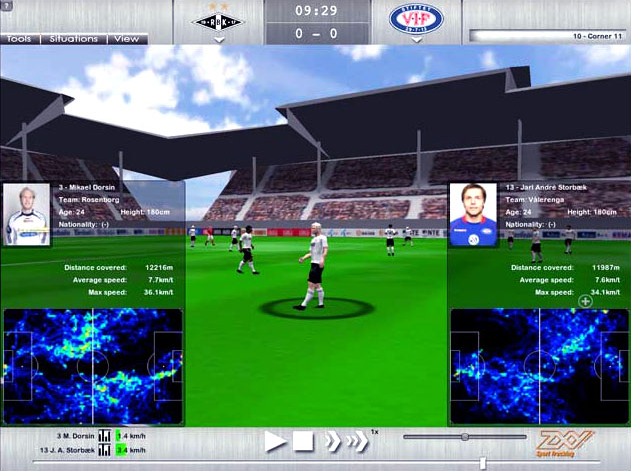
\includegraphics[width=1\textwidth]{images/general/zxysoftware.png}
\caption{The ZXY software - tracking of players gives you information of distance covered, average speed and max speed. You also get a heat map of the players movement on the field. Image from zxy.no}
\label{fig:zxysoftware}
\end{figure}


\subsection{FourFourTwo}

FourFourTwo is a monthly magazine about football. They also have a webpage which they update daily. Particular they focus on analytic and has a business del with Opta giving them access to all theirs statistics. Including to own analyses on their page they have their own application Stats Zone where everyone can analyze matches with the same tools as they do self. Figure \ref{fig:fourfourtwo} shows a typical
graphical illustration done with the Stats Zone application highlighting passes in to attacking third. 

\begin{figure}[ht!]
\centering
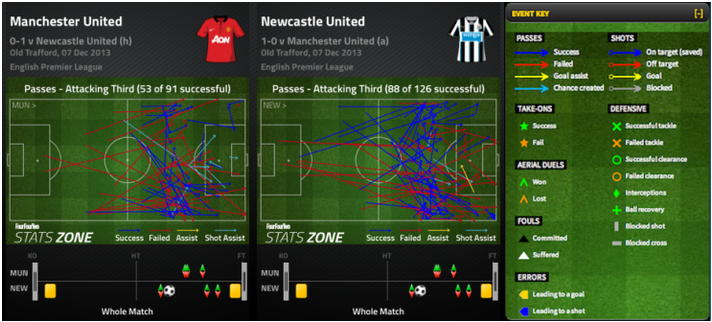
\includegraphics[width=1\textwidth]{images/general/fourfourtwo.png}
\caption{Illustration of all passes in to attacking third in the match Manchester United vs Newcastle United. Taken from fourfourtwo.com}
\label{fig:fourfourtwo}
\end{figure}